%Zarantonello Umberto 20/04/21

\section{Il Nucleo}
\subsection{Le scoperta delle particelle nucleari}
La seconda particella ad essere rivelata dopo l'elettrone fu il protone. 
La prima evidenza sperimentale è dovuta sempre a Rutherford che nel 1917, sfruttando sempre le particelle alfa in collisione con l'aria, riuscì ad ottenere delle emissioni protoniche. La reazione che si verificava era la seguente (l'aria viene approssimata con l'azoto $N$) 
\begin{equation}
^4_2He +^{14}_{7}N_{7}\longrightarrow ^{17}_8O_9+protone
\end{equation}
Al tempo uno modelli nucleari più in voga teorizzava un nucleo composto da un certo numero $A$ di protoni ed un numero $A-Z$ di elettroni, dove $Z$ è il numero di elettroni della nuvola elettronica.
Questo modello generava un atomo neutro e stabile ed era dovuto principalmente al fatto di non aver ancora scoperto il neutrone che è necessario alla stabilità del nucleo (non ci si spiegava come si potesse bilanciare l'elevata forza repulsiva dei protoni all'interno del nucleo).

Analizziamo dunque la possibilità di avere un nucleo di questo tipo.
Che potenziale elettromagnetico dovrebbero gestire i protoni?

Il campo elettrico che si genera è
\[E=\frac{Ze^2}{4\pi\varepsilon_0R}\]
dove $R=R_0 A^{1/3}=1.2fm\cdot A^{1/3}$ (formula empirica per il calcolo del raggio nucleare). 
Calcolando si ottiene quindi
\[E=-1.20\frac{Z}{A^{1/3}MeV}\]

Ponendo ora per esempio A=140 e Z=58 l'energia cinetica che si ottiene è $E=-13.4MeV$ (elettrone con energia relativistica quindi $E=pc$). Un elettrone con tale energia cinetica è possibile che resti confinato all'interno del nucleo?

Prendiamo quella che è la lunghezza d'onda dell'elettrone
\[\lambda=\frac{h}{p}=2\pi \frac{\hbar c}{pc}=\frac{2\cdot 3.14\cdot 200MeV\cdot fm}{13.4MeV}\simeq 90fm\]
Se si considera che il raggio calcolato da Rutherford era di $46fm$ è evidente che l'elettrone non può essere confinato nel nucleo perché la sua lunghezza d'onda è il doppio.

\paragraph{La scoperta del neutrone} fu fatta da Chadwick che fu il primo ad intuire, da un'esperienza che in realtà era già stata fatta da più fisici, la presenza di un'altra particella. 
La situazione che si verificava era che tramite l'emissione di particelle alfa generate dal polonio, fatte collidere su un target di Berilio, si otteneva una radiazione che riusciva ad attraversare uno schermo spesso di piombo, il che suggeriva il fatto che fosse una radiazione neutra (impossibile per della radiazione carica attraversare uno schermo troppo spesso). 
Al tempo l'unica radiazione neutra conosciuta era la radiazione elettromagnetica il che fece pensare ad una reazione del tipo
\[
^9_4Be+^4_2He\longrightarrow[^{13}_6C*]\longrightarrow^{13}_6C+\gamma
\]
Con uno stato intermedio dato da uno stato eccitato del carbonio 13.

Un ulteriore passaggio fu quello di aggiungere dopo lo schermo di Piombo $Pb$ una lastra di paraffina da cui, dopo l'interazione con la radiazione, emergevano protoni con energia pari a $E=7,5MeV$. 
La radiazione gamma doveva quindi possedere un'energia in grado di produrre dei protoni di energia $7,5MeV$ tramite scattering Compton il che riconduce ad un'energia minima di $55MeV$.
Quando il Berilio assorbiva le particelle alfa queste si trovavano ad un energia di $5MeV$, essendo poi una reazione esotermica si aveva che il Q della reazione corrispondeva a $Q=10MeV$, il che riconduceva ad un energia massima disponibile di $14MeV$.
L'unica spiegazione possibile era che si trattava quindi di una particella nuova, neutra e con la stessa massa del protone.
Era stato scoperto il neutrone.

%nuova sezione-------------------------------------------------------------
\subsection{Studio dei nuclei: diffusione elastica elettrone nucleo}
Per superare i limiti dati dallo studio con le particelle Alfa, attorno agli anni '50 si cominciarono a sfruttare gli elettroni come sonda.
L'utilizzo di questo tipo di particelle avvenne così tardi non perché non se ne conoscessero i vantaggi ma vi è la necessità di acceleratori per portare gli elettroni ad un'energia abbastanza elevata.
Questi sono stati la sonda "principe" per lo studio del nucleo ma anche dei nucleoni (protoni e neutroni), perché:
\begin{itemize}
\item possono essere considerati puntiformi, infatti per quanto ne sappiamo non possiedono struttura, e quindi le loro dimensioni non impattano nello studio del nucleone.
\item interagiscono solo per interazione elettromagnetica, a differenza per dire delle particelle alfa che interagiscono anche tramite la forza forte rendendo difficoltosa la distinzione tra i due tipi di interazione.
\end{itemize}

L'innovazione in questo campo è stata data dall'energia a cui si riesce ad accelerare gli elettroni portando a nuove scoperte.

Perché è così importante ottenere energie sempre più elevate per avere maggiore risoluzione sulla struttura?
Il motivo si basa sulla relazione di de Broglie, infatti quando si vuole studiare la struttura, la lunghezza d'onda della sonda deve essere più piccola della struttura che andiamo a studiare.
\begin{equation}
\begin{split}
\lambda=\frac{h}{p}&\leq 2R\\
\frac{2\pi\hbar}{p}&=2R\\
pc&=\frac{2\pi\hbar}{2R}
\end{split}
\end{equation}
Siccome gli elettroni necessitano di una bassa energia per diventare relativistici (ovvero per avere una velocità prossima a quella della luce e quindi energia indipendente dalla massa), gli elettroni usati come sonda sono quasi sempre relativistici. Per questo la formula sopra può essere riscritta sfruttando l'equazione di Einstein per l'energia.
\begin{equation}
\begin{split}
E^2 &=p^2c^2+m^2c^4\\
p^2c^2 \gg m^2c^4 &\hspace{0.5cm}\to\hspace{0.5cm}E=pc
\end{split}
\end{equation}
Si ottiene quindi che l'energia degli elettroni deve essere pari a 
\begin{equation}
E=2\pi\frac{197MeV\cdot fm}{2R}
\end{equation}
Per completare la trattazione si sa già dalle formule sperimentali che il raggio del nucleo si ottiene tramite la formula
\begin{equation}
r_{nucleo}=r_0A^{1/3}
\end{equation}
che, come già visto nel caso dell'oro è $r_{Au}=1.2\sqrt[3]{197}=6,98 fm$.
Il che corrisponde ad un'energia di
\begin{equation}
pc=\frac{2\pi\cdot 197MeV\cdot fm}{2\cdot6,98}=89MeV
\end{equation}
Se quindi voglio usare gli elettroni per studiare questo tipo di nucleo dovrò accelerare gli elettroni ad un minimo di $89 MeV$.

Aumentando ulteriormente l'energia si può ottenere una diminuzione della lunghezza d'onda che aumenta la risoluzione del sistema rendendo visibili i nucleoni.
Ciò che cambia nello studio dei nucleoni rispetto al nucleo è che non si può più considerare elastica la collisione il che porta nella maggior parte dei casi ad una distruzione del protone dopo la collisione e di conseguenza cambierà anche la sezione d'urto.
L'energia necessaria per lo studio del protone ($r_{prot.}\sim 1fm$) è $E=pc=0,5GeV$.
Aumentando ancora l'energia si possono studiare pure i quark, questo richiede energie pari a 6,1 TeV.

%nuova sezione-------------------------------------------------------------
\subsection{Sezione d'urto di Mott}
Le assunzioni fatte per il calcolo della sezione d'urto di Rutherford sono state:
\begin{enumerate}
\item Interazione puramente coulombiana
\item Ne proiettile ne bersaglio possiedono spin
\end{enumerate}
Le assunzione su cui si baserà la sezione d'urto di Mott, necessaria alla descrizione dell'interazione nucleo elettrone, sono:
\begin{enumerate}
\item Bersaglio privo di spin
\item Proiettile con spin
\end{enumerate}
Questi cambi, necessari per esperimenti con gli elettroni portano alla formula seguente
\begin{equation}
\left(\frac{d\sigma}{d\Omega}\right)^*_{Mott} =\left(\frac{d\sigma}{d\Omega}\right)_{Ruth}\left(1-\beta^2\sin^2\frac{\theta}{2}\right)
\end{equation}
con $\beta=v/c$.
L'asterisco sta ad indicare che trascuriamo gli effetti di rinculo.

Si continua a supporre quindi che il nucleo abbia massa infinita e di conseguenza che l'elettrone abbia energia cinetica iniziale uguale a quella finale.
Questa assunzione è possibile fino al GeV perché al di sopra le quantità di moto di elettrone e nucleo iniziano a diventare confrontabili.
Il termine moltiplicativo della sezione d'urto di Rutherford sopra è ciò che ci indica la presenza dello spin dell'elettrone, studiamo ora il suo significato.
\begin{equation}
\begin{split}
\beta&\to1\\
v&\to c\\
1-\beta^2\sin^2\frac{\theta}{2}&\to \cos^2\frac{\theta}{2}
\end{split}
\end{equation}
Questo comporta una grande modifica alla sezione d'urto di Rutherford, in quanto viene inibito il back scattering caratteristico dell'esperimento con il bersaglio d'oro, e ciò è dovuto proprio allo spin dell'elettrone.
Questo ci fa capire quanto sia stato fortuita scelta di Rutherford delle particelle $\alpha$ che non provocano appunto interazione di spin.

Questo effetto si spiega grazie ad una quantità caratteristica di ogni particella definita elicità
\begin{equation}
h=\frac{\bar s\cdot \bar p}{|s||p|}
\end{equation}
Questa grandezza, come si può intuire dalla formula è la proiezione dello spin nella direzione della quantità di moto.
Lo spin è una proprietà caratteristica delle particelle che classicamente viene rappresentata come una rotazione della particella attorno a se stessa. Questa è un'immagine molto utile a comprendere il concetto ma scorretta da un punto di vista reale (l'elettrone puntiforme e quindi non ha alcun senso parlare di rotazione attorno ad un asse).

\begin{figure}[h]
\centering
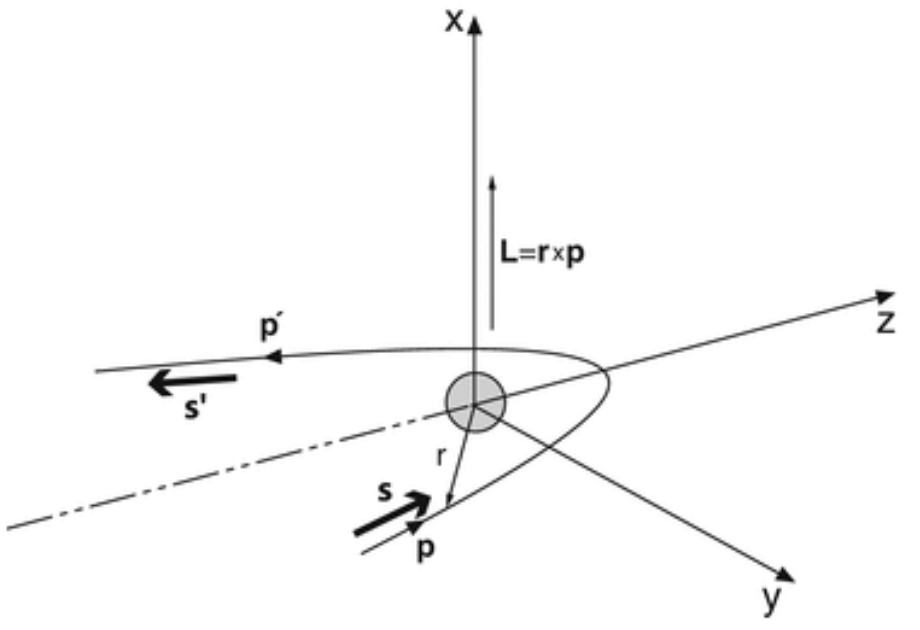
\includegraphics[width=180pt]{fig2_01}
\caption{Backscattering di elettrone}
\label{fig:2.01}
\end{figure}
In figura è mostrata l'interazione tra il nucleo e l'elettrone in cui si ha la conservazione del momento angolare e dell'elicità.
Questo proibisce il back scattering infatti per la conservazione della quantità di moto un evento di back scattering richiederebbe un'inversione dell'elicità, ma siccome anche l'elicità dell'elettrone si deve conservare l'effetto risulta inibito.

La conservazione dell'elicità dipende da regole naturali e riguarda le particelle con velocità prossime a quella della luce.
Una spiegazione che può aiutare alla comprensione è quella di considerare una particella con velocità non relativistica; questa particella può essere osservata sia stando dietro la particella che superandola e guardandola dal fronte, questo genera un cambio di elicità.
La questione è abbastanza intuitiva, basta ragionare con l'esempio di una sfera che ruota attorno a sé stessa in un sistema fisso, questa girerà in senso orario o antiorario in base al punto in cui la si osservi.
Nel caso invece in cui la particella ha velocità tendente a quella della luce l'elicità è definita in quanto la particella non potrà essere vista idealmente da nessun'altra posizione (la particella non potrà mai essere superata).
L'elicità in questo caso viene denominata chiralità.
\begin{figure}[h]
\centering
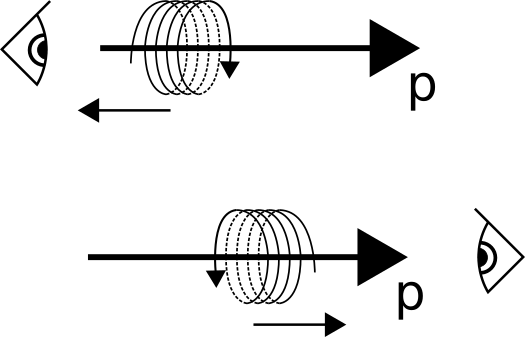
\includegraphics[width=150pt]{fig2_06}
\caption{Rappresentazione grafica del cambio di elicità}
\end{figure}

Ciò vuol dire che gli elettroni possiedono più componenti di elicità ma quando si avvicinano a velocità relativistiche ne rimane solamente una. Questa è una legge che deriva dall'esperienza, non ha quindi un motivo se non l'osservazione.
\'E inoltre un'evidenza dell'equazione di Dirac e da osservazioni della forza debole.
Questo indica che la natura non è simmetrica e ci deve andare bene (la materia preferisce chiralità sinistra, l'antimateria la destra).

In realtà un modo per far cambiare spin e quindi elicità alle particelle ci sarebbe ma richiede la presenza di una campo magnetico, il campo elettrico non è sufficiente. Questo aggiunge un'altra negazione alla possibilità di back scattering. 

%nuova sezione-------------------------------------------------------------
\subsection{Studio dell'interazione sonda bersaglio}
\begin{figure}[h]
\centering
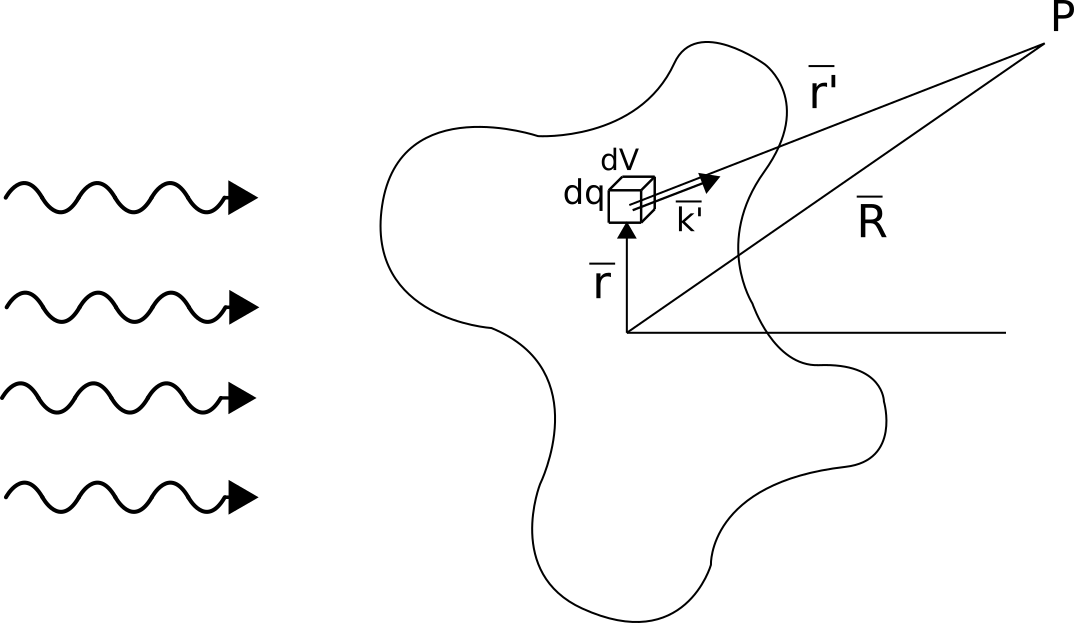
\includegraphics[width=250pt]{fig2_02}
\caption{Rappresentazione dell'interazione di un fascio con una distribuzione di carica}
\label{fig:2.02}
\end{figure}

Supponiamo di avere un fascio di elettroni incidenti su un bersaglio esteso.
Il fascio di elettroni può essere rappresentato come un'onda piana $e^{ikr}$, si consideri che il bersaglio abbia una distribuzione di carica qualsiasi e si prenda un sistema di coordinate centrato al centro della carica.

L'interazione che si ottiene può essere vista come la somma di tutte le interazioni derivate dai punti infinitesimi della carica. 
Per visualizzare questo si consideri un cubetto di carica $dq$ e volume $dV$, con coordinata $\bar r$ rispetto al centro di coordinate. 
Analogamente a come si fa in ottica, supponiamo che dopo l'interazione si generi da quel punto un'onda sferica.

A questo punto è possibile analizzare l'onda ottenuta nel punto P (virtualmente considerato all'infinito) di coordinata $\bar{R}$ rispetto al centro del nucleo e con distanza $\bar{r'}$ rispetto al volumetto infinitesimo di carica.
Si può quindi sommare il contributo di ogni carica infinitesima per ottenere il contributo totale nel punto P dato da tutto il nucleo.
Prendendo come onda piana incidente un'onda di energia:
\begin{equation}
E=E_0\cdot e^{ikr}
\end{equation}
il contributo infinitesimo dell'onda generata è rappresentato da
\begin{equation}
A=E_0 e^{ikr}\frac{a}{r'}e^{ik'r'}=\frac{aE_0}{r'}e^{i(kr+k'r')}
\end{equation}
dove $a$ è l'ampiezza di diffusione, ovvero la sezione d'urto elementare di Mott.
\begin{equation}
\begin{split}
\bar{r}+\bar{r'}&=\bar{R}\\
\bar{k}\bar{r}&=\bar{k'}\bar{R}-\bar{k'}\bar{r'}\\
\end{split}
\end{equation}
Applichiamo quindi delle approssimazioni per semplificare il sistema
\begin{equation}
\begin{split}
R\to\infty &\hspace{0.5cm}r'\approx R\hspace{0.5cm}k'||R\\
M_{nucleo}\to\infty &\hspace{0.5cm}|k'|=|k|=k
\end{split}
\end{equation}
Sostituendo nella formula di $A$ si trova
\begin{equation}
A=\frac{aE_0}{R}e^{ikR}\cdot e^{i(k-k')r}
\end{equation}
Integrando poi su tutto il volume
\begin{equation}
\int A=\frac{aE_0}{RQ}\int \rho_e(r)e^{-i\Delta kr)}
\end{equation}
Dove $Q$ è la carica totale e $\rho$ è la densità di carica.
\'E già noto che la quantità di moto trasferita si può riscrivere come
\begin{equation}
\bar{q}=\hbar \bar{\Delta K}
\end{equation}
\begin{equation}
\int A=\frac{aE_0}{RZe}\int \rho_e(r)e^{-i\frac{q}{\hbar}r}
\end{equation}
Essendo $a$ la sezione d'urto di Mott ve ne si può evidenziare la dipendenza cinematica dovuta alla sua dipendenza dalla sezione d'urto di Rutherford ($\propto 1/q^4$). 
Non sarà dimostrato ma bisogna sapere che $d\sigma/d\Omega$ dipende da $|A|^2$.
Si può finalmente trovare la sezione d'urto
\begin{equation}
\begin{split}
\left(\frac{d\sigma}{d\Omega}\right)_\theta &=\left(\frac{d\sigma}{d\Omega}\right)_{Mott}\biggl| \int\rho_e(r)\cdot e^{-i\frac{q}{\hbar}}dr\biggl|^2\\
&=\left(\frac{d\sigma}{d\Omega}\right)_{Mott}|F(\rho,q)|^2
\end{split}
\end{equation}
$|F(\rho,q)|$ è definito fattore di forma nucleare e coincide con la trasformata di Fourier della distribuzione di carica nel nucleo.
\begin{equation}
F(\rho, q)=\int \rho_e(r)e^{-i\frac{q}{\hbar}r}dr
\end{equation}
In pratica quando un fascio di elettroni interagisce con una densità di carica di ottiene o stesso effetto che si ha con un'onda piana che fa diffrazione da una fenditura.

\paragraph{Esempi}
In figura è mostrato un esperimento di scattering dove c'è un fascio interagente con un bersaglio rivelato da uno spettrometro magnetico rotante che poteva misurare l'energia delle particelle a più angoli di diffusione. Il grafico ottenuto da un'esperienza di questo tipo è mostrato in figura ~\ref{N:01}.
\begin{figure}[h]
\centering
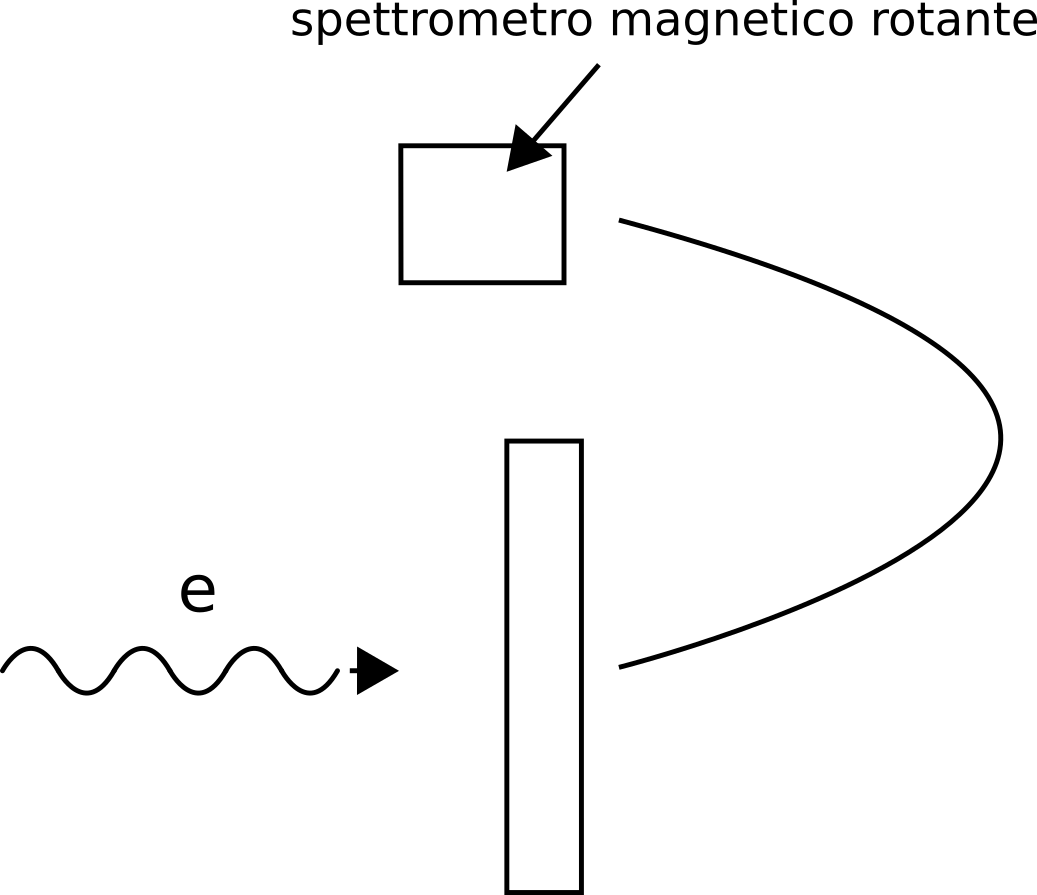
\includegraphics[width=150pt]{fig2_03}
\end{figure}

Come si può notare dal grafico la distribuzione di carica era in un certo modo inaspettata ma rispecchia i ragionamenti fatti riguardo la variabilità della sezione di Mott in base alla distribuzione.
La distribuzione di Mott infatti viene modulata come la trasformata di Fourier della distribuzione di carica e se, per esempio, la distribuzione di carica fosse puntiforme sarebbe uguale alla delta di Dirac, non avendo nessuna deviazione dalla sezione di Mott prevista, in quanto la trasformata di una delta è una distribuzione uniforme. 
\begin{figure}[h]
\centering
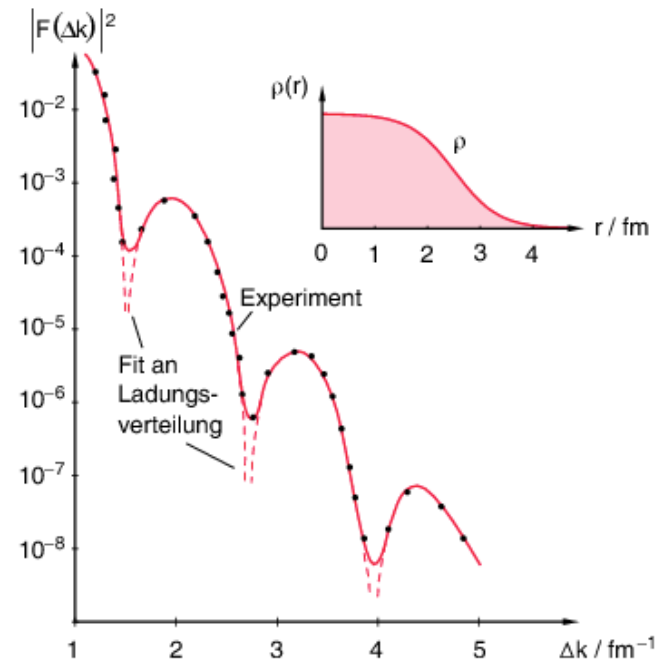
\includegraphics[width=180pt]{fig2_04}
\caption{Risultati sperimentali sfruttando come sonda gli elettroni e che evidenziano l'analogia con l'ottica}
\label{N:01}
\end{figure}

Dai dati sperimentali si ottenne però il grafico ~\ref{N:01}, dovuto al fatto di non poter considerare il nucleo come puntiforme.
Come si può notare, i dati sperimentali evidenziano un importante parallelismo con l'effetto di diffrazione della luce su una fenditura.

Questo rende possibile la determinazione del raggio del nucleo sfruttando le stesse formule usate per trovare la dimensione di una fenditura.
Si prenda per esempio un nucleo di Stagno $^{124}Sn$ e vi si faccia collimare un fascio di elettroni con energia $E=330MeV$;
il raggio del nucleo sarà
\begin{equation}
r=0,61 \frac{\lambda}{\sin\theta}
\end{equation} 
La lambda corrisponde a $\lambda=hc/E=3,7fm$ e il primo minimo si trova a $\theta=45^o$, si ottiene quindi un raggio pari a $r=3,19fm$.

Questi esperimenti ci hanno permesso di determinare la distribuzione di carica del nucleo, che corrisponde all'incirca alla distribuzione di massa.
Ciò che si è notato è che il nucleo non è propriamente una sfera rigida ma ha un andamento come quello mostrato in figura sotto.
\begin{figure}[h]
\centering
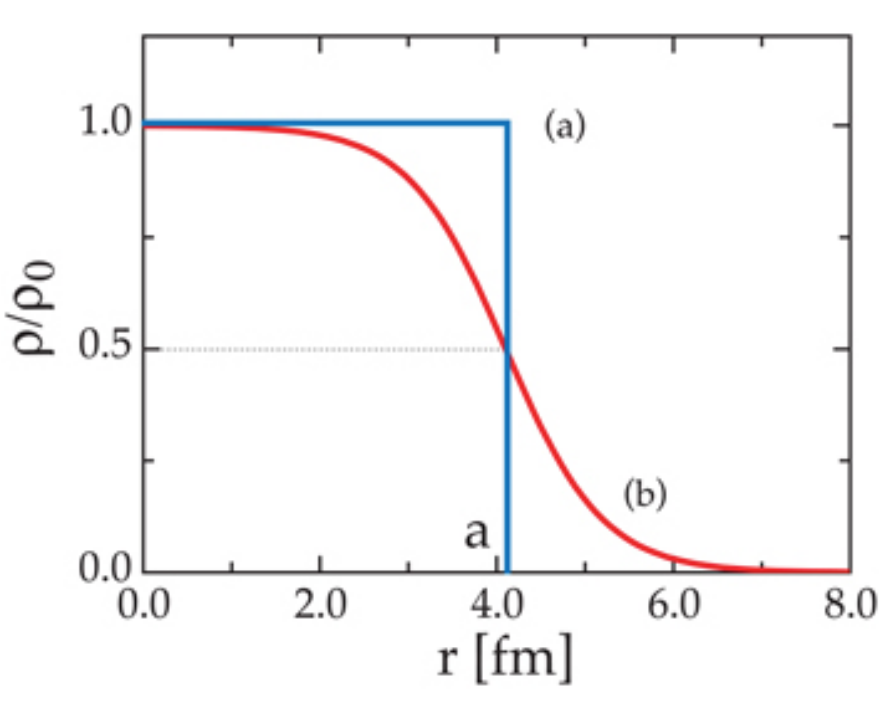
\includegraphics[width=150pt]{fig2_05}
\end{figure}
Questa corrisponde alla distribuzione di Saxon-Woods data dalla formula
\begin{equation}
\rho(r)=\frac{\rho_0}{1+exp\left(\frac{r-a}{b}\right)}
\end{equation}
dove $a=118A^{1/3}=0,48fm$ e $b=0,55\pm 0,07fm$.
Questo mostra la presenza di una zona dove la densità del nucleo diminuisce gradualmente.

Qual è la densità di materia nel nucleo?
\begin{equation}
\begin{split}
R&=R_0A^{1/3}\\
\rho_{M}&=\frac{M}{V}=\frac{A\cdot u}{\frac{4}{3}\pi R^3}\\
&=\frac{A\cdot u}{\frac{4}{3}\pi R_0^3A}\approx10^{17}\frac{kg}{m^3}
\end{split}
\end{equation}
dove $A$ corrisponde al numero di massa del nucleo e $u$ è l'unità di massa atomica. 
Dalla divisione di A per A si nota come la densità non dipende dal tipo di nucleo ma è uguale per tutti i nuclei.


%nuova sezione--------------------------------------------------
\subsection{Proprietà dei Nuclei: Spin Nucleare e Momento Magnetico}
Molte proprietà dei nuclei si caratterizzano in modo fenomenologico, ovvero per analogia con effetti già conosciuti.
Lo spin viene descritto in analogia a ciò che viene studiato in struttura della materia e meccanica quantistica. 
Ricordiamo ora com'è caratterizzato il moto dell'elettrone attorno al nucleo, questo si descrive come un moto di rivoluzione e di rotazione.
\begin{figure}[h]
\centering
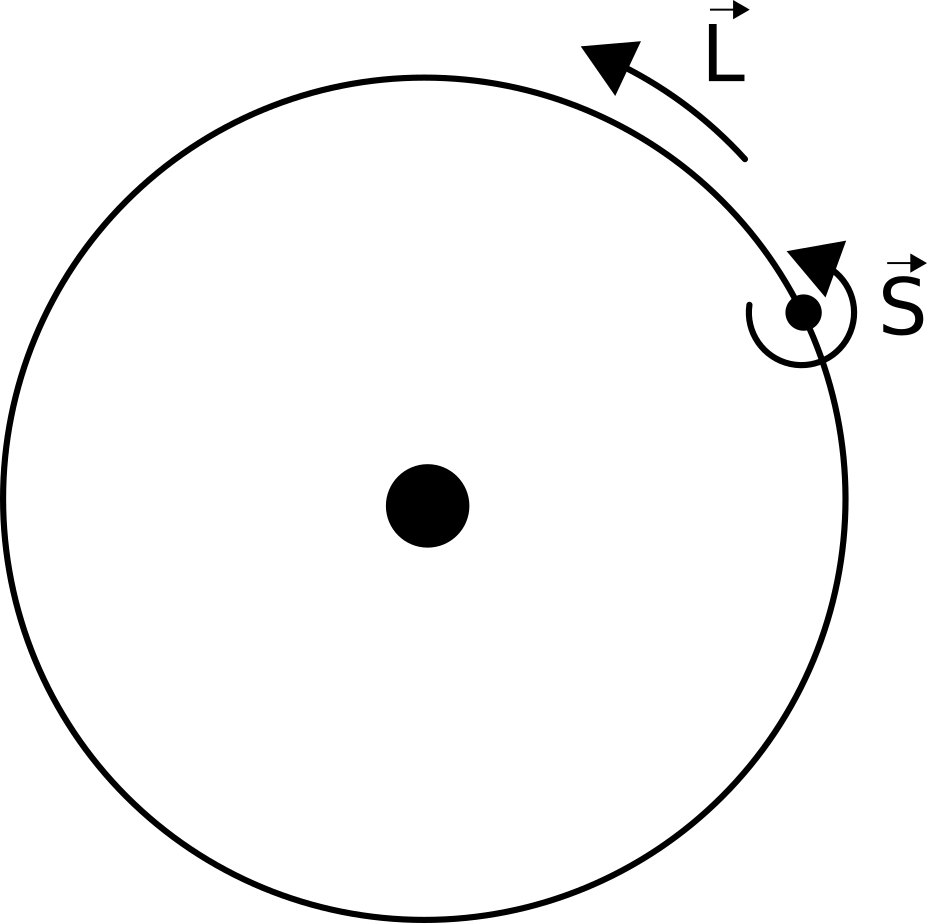
\includegraphics[width=130pt]{fig3_01}
\end{figure}

Vi sono inoltre più numeri quantici che caratterizzano l'elettrone:
\begin{equation}
\begin{split}
n\hspace{1cm} & 1, 2,3\\
l\hspace{1cm} & 0\to N-1\\
m\hspace{1cm} & -l\to0\to+l\\
s\hspace{1cm} & +\frac{1}{2}, -\frac{1}{2}
\end{split}
\end{equation}
Per quanto riguarda i nucleoni, il fatto di avere un momento angolare non è banale, non vi è infatti un potenziale centrale che ne giustifichi la presenza.
La questione è valida in quanto dimostrata da fatti sperimentali.
Per ogni nucleone, all'interno del nucleo, possiamo definire un momento angolare totale che è dato da 
\begin{equation}
\bar s =\bar l + \bar s
\end{equation}
e con lo stesso tipo di analogia potremo trovare quello che si chiama spin del nucleo, ottenuto come la somma di tutti gli spin dei nucleoni.
\begin{equation}
I=\sum \bar s
\end{equation}
La spiegazione deriva dal fatto che siccome i protoni sono particelle cariche, e una particella carica in moto genera un momento magnetico, si otterrà anche per i nucleoni un momento magnetico.

\paragraph{un paio di commenti}
\begin{itemize}
\item L'analogia dello spin di una particella con una trottola è una assunzione ben posta?
Si parte dal raggio classico dell'elettrone, ovvero il raggio che una carica avrebbe se tutta la sua massa fosse costituita da energia elettrostatica.
\begin{equation}
\begin{split}
m_e c^2=\frac{1}{4\pi\varepsilon_0}\frac{e^2}{r_e}\hspace{0.2cm}\to\hspace{0.2cm}r_e & =\frac{1}{4\pi\varepsilon_0}\frac{e^2}{m_ec^2}=\\
&=\frac{e^2\hbar c}{4\pi \varepsilon_0\hbar c}\frac{1}{m_ec^2}=\\
&=1,44MeV\cdot fm\frac{1}{0,5MeV}\sim 3fm
\end{split}
\end{equation}
In realtà noi consideriamo l'elettrone come una particella priva di struttura il che ci fa capire quanto sbagliata sia la nostra concezione di questi fenomeni. 
Il raggio reale è approssimabile a $0$.
Supponiamo che il momento angolare dell'elettrone sia \emph{(consideriamo qui l'elettrone come una sferetta con tutta la massa concentrata al bordo della sfera)}:
\begin{equation}
\hbar=r_e m_e v_e
\end{equation}
Qual è la velocità di questa sfera (elettrone)?
\begin{equation}
\begin{split}
v_e&=\frac{\hbar}{r_em_e}\to\frac{v_e}{c}\\
&=\frac{\hbar c}{r_em_e^2}\sim 10^2
\end{split}
\end{equation}

Il risultato ottenuto è assurdo, perché viola le regole base della relatività. 
L'analogia con la trottola è quindi un espediente utile alla comprensione ma errato e lo spin è da considerarsi un effetto puramente relativistico.
\item Qual è il cammino libero medio del nucleone nel nucleo?
Si ha
\begin{equation}
l=\frac{1}{n\delta}
\end{equation}
dove $\delta_{n-n}\sim 22MeV=300 mb$ è la sezione d'urto d'interazione e $n$ è alla densità numerica dei nucleoni nel nucleo.
\begin{equation}
n=\frac{A}{V}=\frac{A}{\frac{4}{3}\pi R_0^3 A}=\frac{3}{4(3,14)(1,15fm)^3}=0,16\frac{nucleoni}{fm^3}
\end{equation}
Il libero cammino medio sarà quindi
\begin{equation}
l=\frac{1}{0,16fm^3}\frac{1}{300\times 10^{-3}\cdot10^{-28}m^2\cdot 10^{30}fm^2/m^2}=0,21fm
\end{equation}
Il libero cammino medio corrisponde quindi a meno della dimensione del nucleone stesso, il che non fa ben sperare alla possibilità di spostamento dei nucleoni e alla conseguente esistenza di un momento magnetico.
In realtà c'è possibilità di movimento grazie al principio di esclusione di Pauli.
\end{itemize}

Dal punto di vista sperimentale quello che noi vediamo è che i nuclei hanno un certo momento magnetico (rather than l'effetto del momento angolare).
\begin{figure}[h]
\centering
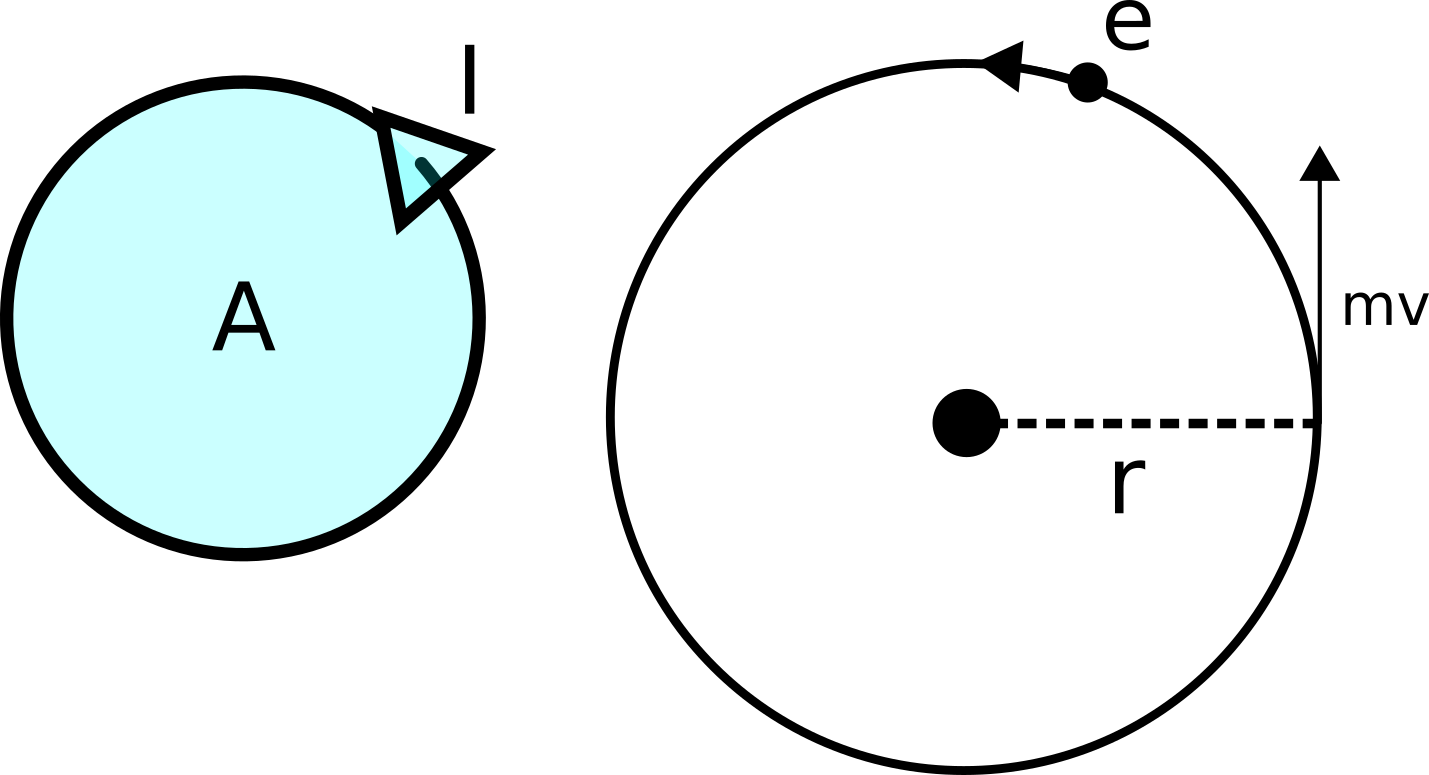
\includegraphics[width=200pt]{fig3_02}
\end{figure}
Il momento magnetico associato ad una carica in moto classicamente corrisponde alla corrente che attraversa una spira per l'area della spira stessa.
\begin{equation}
\mu=IA
\end{equation}

Prendendo ora il caso dell'elettrone (che poi sarà ampliato per analogia al caso dei nucleoni) si ha 
\begin{equation}
L=mvr, \hspace{0.5cm}I=\frac{e}{v}
\end{equation}
\begin{equation}
v=\frac{2\pi r}{t}\to t=\frac{2\pi r}{v}
\end{equation}
Si ottiene così la corrente generata da un elettrone
\begin{equation}
I=\frac{e}{2\pi r}v
\end{equation}
il che può essere sostituito nel momento magnetico per ottenere
\begin{equation}
\mu=IA=\frac{e}{2\pi r}v\pi r^2=\frac{evr}{2}\frac{mvr}{mvr}=\frac{e}{2m}L
\end{equation}
Il \emph{momento magnetico} di una particella carica è quindi
\begin{equation}
\mu=\frac{e}{2m}L
\label{PN:02}
\end{equation}
Dove la quantità $e/2m$ viene definita come \emph{rapporto giromagnetico}. 
Il momento ~\eqref{PN:02} fa riferimento alla meccanica classica ma può essere validato per la meccanica quantistica effettuando la sostituzione del momento angolare con $\hbar$.
Si ottiene così il \emph{magnetone di Bohr}
\begin{equation}
\mu_B=\frac{e}{2m_e}\hbar
\end{equation}
Questa è l'unità fondamentale per quanto riguarda il momento magnetico.
Possiamo poi ampliare questa definizione trovando il momento di dipolo magnetico dell'elettrone
\begin{equation}
\mu_e =\mu_B \frac{L}{\hbar}
\label{PN:01}
\end{equation}
Si può ora introdurre il fattore giromagnetico $g$ che ci permette di generalizzare la formula ~\eqref{PN:01}
\begin{equation}
\mu_B =g\mu_B \frac{L}{\hbar}
\end{equation}
A questi livelli di grandezza non si ha la certezza che carica e massa coincidano, anzi potrebbero essere totalmente indipendenti; questo fattore assume che ci sia una relazione ben definita tra momento angolare e momento magnetico, in particolare se distribuzione di massa e di carica coincidono $g=1$.
La trattazione ha comunque dei limiti, infatti quando verrà studiato lo \emph{spin} del nucleo si potrà notare come massa e carica non coincidano, ma per ora va bene che ci siano dei limiti nel calcolo.
Nel caso dell'elettrone che gira attorno al nucleo è vero che $g=1$.

Nel caso dei nucleoni all'interno del nucleo si ha per il protone:
\begin{equation}
\mu_p=\mu_N\frac{L}{\hbar}\hspace{1cm}\mu_N=\frac{e\hbar}{2m_p}
\end{equation}
dove $g=1$ e $\mu_N$ è detto magnetone nucleare.
Mentre per il neutrone:
\begin{equation}
\mu_n=0
\end{equation}

Per quanto riguarda lo \emph{spin} si ha che la relazione diventa
\begin{equation}
\mu_e=g\mu_B \frac{S}{\hbar}
\end{equation}
In questo il momento giromagnetico non sarà più $1$ ma si avrà $g_e=2$.
Questo valore si ottiene dall'equazione di Dirac per particelle prive di struttura interna.
Dall'elettrodinamica quantistica si ottiene poi che in realtà non è propriamente 2 ma $g=2,0023$ che coincide con una piccola variazione ma che deriva da cambiamenti importanti (tanto da essere scritta sull'epitaffio dello scopritore).
Nel caso dei nucleoni si ha
\begin{equation}
\mu_{p,n}=g_{p,n}\mu_N\frac{S}{\hbar}
\end{equation}
dove i fattori g corrispondono a $g_p=5,585691; g_n=-3,826084$.
Il fatto che questi fattori siano diversi da 2 ci fa capire come i nucleoni abbiano entrambi una struttura interna; si ha inoltre che il $g\not0$ per il neutrone implica che pure quest'ultimo possieda un momento magnetico pur essendo privo di carica.

Il momento di dipolo magnetico totale del nucleo è
\begin{equation}
\mu_N=\sum_p \left(\mu_N \frac{\bar{L}}{\hbar}+g_p\mu_N\frac{\bar S}{\hbar}\right)+\sum_n \biggl[g_n \mu_N\frac{\bar S}{\hbar}\biggl]
\end{equation}
\begin{figure}[h]
\centering
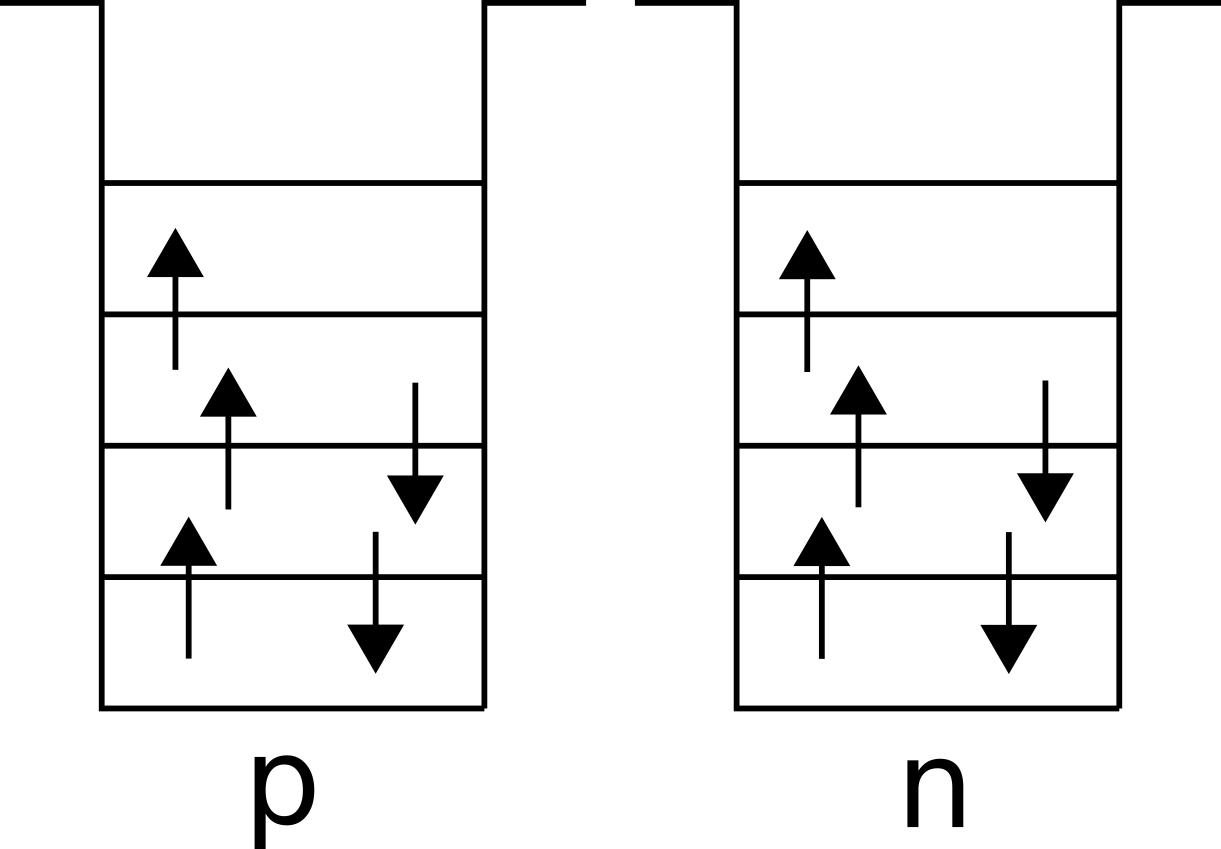
\includegraphics[width=180pt]{fig3_03}
\caption{Rappresentazione delle buche di potenziale dei protoni e dei neutroni}
\end{figure}
Una cosa interessante riguardo i neutroni e i protoni è che queste particelle sono fermioni ovvero particelle che soddisfano alla statistica di Fermi-Dirac (non posso avere più di una particella nello stesso stato, posso avere al massimo due particelle alla stessa energia con spin antiparallelo).
Essendo poi particelle all'interno di una buca di potenziale si può già intuire quale sarà lo spin del nucleo.
Per esempio:
\begin{itemize}
\item se il numero di massa A è pari e il numero atomico Z è dispari, avremo un numero dispari di neutroni e di protoni, in questo caso il nucleone spaiato (sia dalla parte dei neutroni che dei protoni) mi fa dire che avremo un nucleo con spin intero.
\item Se invece il numero totale di nucleoni è pari e il numero di protoni e neutroni è pari si avrà spin del nucleo nullo.
\item Se il numero di massa sarà dispari sappiamo che lo spin del nucleo è semi-intero.
\end{itemize} 